% SPDX-License-Identifier: CC-BY-4.0
% Copyright (c) 2026 Martin Schröder <info@swedishembedded.com>

\section{Measurement protocol}\label{sec:protocol}

This protocol was fixed before any measured run (see also \code{prereg/protocol.md}).
Changes after the first measured run are dated amendments, and results obtained
under a changed rule are labelled post hoc.

\paragraph{Units and arms.} The experimental unit is the \emph{family}: the group of
tasks derived from one mutated path or source entity. Tasks within a family are not
independent, so no test treats them as such. The \emph{base} arm is the unmodified
checkpoint in the pinned harness; the \emph{adapter} arm is the same checkpoint with the
adapter attached; nothing else differs (system prompt, tool schemas, budgets, seeds per
(task, attempt), environment image).

\paragraph{Family outcome and primary test.} For a family, each arm's score is the fraction
of its tasks resolved. The adapter \emph{wins} a family when its score is higher than the
base's and \emph{loses} when lower; tied families are dropped. The primary decision is the
one-sided exact sign test on the non-tied families at $\alpha=\alphalevel$ (the same
test the release gate already uses on paired outcomes). A result that is not significant
is reported as \emph{not shown}, never as equivalence.

\paragraph{Secondary measures (descriptive).} Pooled task-level resolve rate with a
family-cluster bootstrap interval; valid tool-call rate; tool calls and tokens per
resolved task; changed files per patch; environment failures, which are excluded from the
denominator but always reported with their count.

\paragraph{Retention.} After each round $k$, the exam families of every earlier round are
solved again by the round-$k$ adapter and by the round-$(k{-}1)$ adapter. Retention
is supported only if the one-sided $95\%$ lower bound on
$\text{rate}_k-\text{rate}_{k-1}$ (family-cluster bootstrap) exceeds $-\delta$, with
$\delta=0.05$ absolute fixed in advance. Failure of retention is reported as such.

\paragraph{Experiments.} E1: plumbing; train on a few records and require held-out loss on
them to fall and tool-call formatting to stay valid, which shows masks and tool
definitions reach the trainer. E2: one repository, adapter against base. E3: a sequence of
repositories $R_1,R_2,R_3$ with the full matrix of adapter-after-round against exam of each
repository (\cref{fig:matrix}); off-diagonal cells distinguish learning a repository from
learning the tool protocol. E4: a later revision of $R_1$ with new tasks and a continued
adapter. A1: training on all trajectories regardless of verdict. A2: no replay of earlier
repositories.

\begin{figure}[t]
\centering
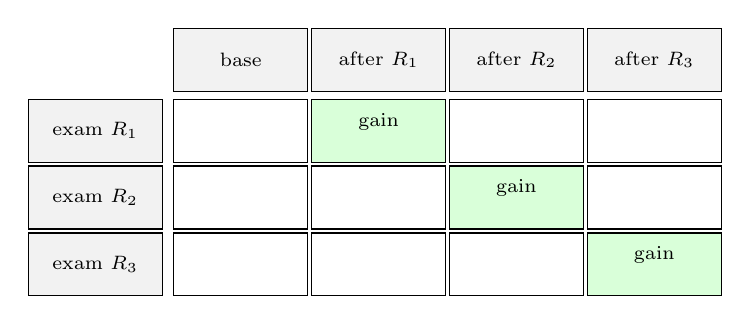
\begin{tikzpicture}[cell/.style={draw,minimum width=1.7cm,minimum height=0.8cm,font=\scriptsize,align=center}]
\foreach \c/\name in {0/base,1/after $R_1$,2/after $R_2$,3/after $R_3$}
  \node[cell,fill=gray!10] at (\c*1.75+1.85,0.9) {\name};
\foreach \r/\name in {0/exam $R_1$,1/exam $R_2$,2/exam $R_3$}
  \node[cell,fill=gray!10] at (0,-\r*0.85) {\name};
\foreach \r in {0,1,2}{
  \pgfmathtruncatemacro{\cc}{\r+1}
  \foreach \c in {0,1,2,3}{
    \ifnum\c=\cc
      \node[cell,fill=green!15] at (\c*1.75+1.85,-\r*0.85) {gain\\\notrun};
    \else
      \node[cell] at (\c*1.75+1.85,-\r*0.85) {\notrun};
    \fi
  }
}
\end{tikzpicture}
\caption{E3 result matrix. Shaded: the round that trained on that repository (the
primary gain). Cells to the right of a shaded cell test retention after later rounds; cells to its left
(including the base) test transfer and protocol learning. Nothing is measured yet.}\label{fig:matrix}
\end{figure}

\paragraph{What the test can decide.} \Cref{tab:design} and \cref{fig:power} give, for the
exact one-sided sign test, the discordant families needed and the power at assumed win
probabilities. With fewer than five non-tied families no decision is possible at
$\alpha=\alphalevel$, and a repository that yields fewer than about twenty reserved
families can reveal only large effects; such a result is reported as underpowered.
These are design calculations, not measurements.

\begin{table}[t]
\centering\small
\begin{tabular}{rrrrrr}
\toprule
Discordant & Wins needed & Smallest $p$ & \multicolumn{3}{c}{Power if $P(\text{win})=$} \\
clusters $n$ & for $p\le 0.05$ & (all wins) & 0.7 & 0.8 & 0.9 \\
\midrule
4 & none & 0.062 & 0.00 & 0.00 & 0.00 \\
5 & 5 & 0.031 & 0.17 & 0.33 & 0.59 \\
6 & 6 & 0.016 & 0.12 & 0.26 & 0.53 \\
8 & 7 & 0.0039 & 0.26 & 0.50 & 0.81 \\
10 & 9 & 0.00098 & 0.15 & 0.38 & 0.74 \\
15 & 12 & 3.1e-05 & 0.30 & 0.65 & 0.94 \\
20 & 15 & 9.5e-07 & 0.42 & 0.80 & 0.99 \\
30 & 20 & 9.3e-10 & 0.73 & 0.97 & 1.00 \\
\bottomrule
\end{tabular}

\caption{Exact one-sided sign test at $\alpha=\alphalevel$: wins required and power if each
non-tied family is a win with the stated probability (design calculation).}\label{tab:design}
\end{table}

\begin{figure}[t]
\centering
\begin{tikzpicture}
\begin{axis}[width=0.75\linewidth,height=5.2cm,xlabel={non-tied exam families $n$},
  ylabel={power},ymin=0,ymax=1.02,xmin=2,xmax=40,legend pos=south east,
  legend style={font=\scriptsize},grid=major,
  every axis plot/.append style={thick}]
\addplot[blue,mark=none] table[col sep=comma,x=n,y=q70] {generated/power_curve.csv};
\addplot[red!70!black,mark=none,dashed] table[col sep=comma,x=n,y=q80] {generated/power_curve.csv};
\addplot[green!50!black,mark=none,dotted] table[col sep=comma,x=n,y=q90] {generated/power_curve.csv};
\legend{$P(\text{win})=0.7$,$P(\text{win})=0.8$,$P(\text{win})=0.9$}
\end{axis}
\end{tikzpicture}
\caption{Power of the exact one-sided sign test ($\alpha=\alphalevel$) against the number of
non-tied families. The sawtooth is the discreteness of the test.}\label{fig:power}
\end{figure}

\paragraph{Leakage and contamination controls.} (i) Families are assigned before rollouts.
(ii) Hidden files are absent from the solver's tree; they are materialised only in the
verifier's directory. (iii) An exposure audit scans each trajectory for hidden paths, hidden
content shingles and the state-root path; an exposed experience fails with a counted reason
and is excluded from training and gates. (iv) The isolation level of each run
(\code{container} or \code{none}) is recorded; with \code{none} the audit detects but cannot
prevent. (v) Repositories that may be in the base model's pretraining data are flagged;
the base-arm comparison on the same exam bounds, but does not remove, that effect.
